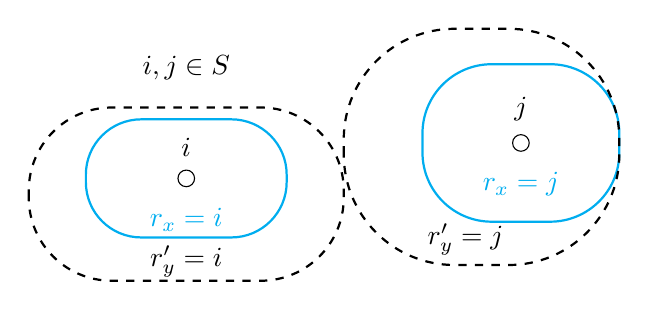
\begin{tikzpicture}

\coordinate (r1) at (2,2.4);
\coordinate (r2) at (6.25,2.85);
\coordinate (r3) at (8,2.8);

\node[] at (2, 3.8) {$i, j\in S$};
\draw (r1) circle [radius=3pt] coordinate (j);
\draw (j) node [above=.15cm] {$i$};
\draw (r2) circle [radius=3pt];
\draw (r2) node [above=.15cm] {$j$};

\node[cyan, draw, shape=rectangle, minimum width=2.55cm, minimum height=1.5cm, anchor=center,rounded corners=20pt,thick] at (r1) {};
\node[cyan] at ([yshift=-15pt]j) {$r_x = i$};
\node [cyan, draw, shape=rectangle, minimum width=2.5cm, minimum height=2.0cm, anchor=center,rounded corners=25pt,thick] at  (r2) {};
\node[cyan] at ([yshift=-15pt]r2) {$r_x = j$};

\draw[\darkorange, rounded corners=30pt,dashed,thick]
  (0,1.1) rectangle ++(4,2.2);
\node[\darkorange] at ([yshift=-30pt]j) {$r'_y = i$};
\draw[\darkorange, rounded corners=40pt,dashed,thick]
  (4,1.3) rectangle ++(3.5,3);
\node[\darkorange] at ([xshift=-20pt,yshift=-35pt]r2) {$r'_y = j$};
\end{tikzpicture}
